\chapter{Speaker Recognition Systems}
\label{ch:speaker-recognition-system}

The process of voice recognition lies on the field of pattern classification, with the speaker's utterance (a speech signal) as input for a classifier and a decision as output. This decision may be, given a speech signal $\boldsymbol{Y}$ produced by a speaker $\mathcal{S}$ and a set $\boldsymbol{\mathcal{S}} = \{\mathcal{S}_1, ..., \mathcal{S}_S\}$ of known users,

\begin{equation}
    \text{classify } \mathcal{S} \text{ as } \mathcal{S}_i \text{ if } i = \arg\max_j P(\mathcal{S}_j|\boldsymbol{Y}).
    \label{eq:decision_speaker_identification}
\end{equation}

\noindent This is a case of speaker identification and the output is a $\mathcal{S}_i$ from $\boldsymbol{\mathcal{S}}$. Another type of decision is

\begin{equation}
    \text{if } P(\mathcal{S}_i|\boldsymbol{Y}) \verifytestB{\alpha}{\mathcal{S} \text{ as } \mathcal{S}_i}
    \label{eq:decision_speaker_verification}
\end{equation}

\noindent a speaker verification decision, with a binary output, given a $\mathcal{S}$ who produced $\boldsymbol{Y}$, a claimed identity $\mathcal{S}_i$ from $\boldsymbol{\mathcal{S}}$ and a threshold of acceptance $\alpha$. This chapter (and indirectly the whole document) is about the type of decision seen in \equationref{decision_speaker_verification}.

\section{Basic Concepts}

\subsection{Utterance}

An utterance is a piece of speech produced by a speaker. It may be a word, a statement or any vocal sound. The terms \emph{utterance} and \emph{speech signal} sometimes are used interchangeably, but from herenow speech signal will be associated to an utterance recorded, digitalized and ready to be processed. An example is shown in \figureref{speech_signal}.

\begin{figure}[ht]
    \centering
    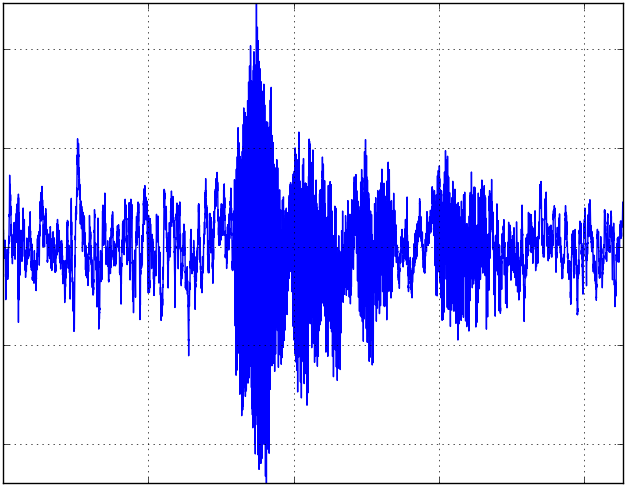
\includegraphics[width=\textwidth]{speech_signal}
    \caption{Speech signal for utterance ``karen livescu", from the MIT dataset \cite{woo.park.hazen.2006}.}
    \label{fig:speech_signal}
\end{figure}

\subsection{Features}

The raw speech signal is unfit for usage by a recognition system. For a correct processing, the unique features from the speaker's vocal tract are extracted, reducing the number of variables the system needs to deal with (leading to a simpler implementation) and performing a better evaluation (and avoiding the curse of dimensionality). Due to the stationary properties of the speech signal when analyzed in a short period of time, it is divided in overlapping frames of small and predefined length, to avoid ``loss of significancy" in the features \cite{davis.mermelstein.1980, rabiner.schafer.2007}. This extraction is executed by the MFCC algorithm, explained in details in \chapterref{feature-extraction}.

\subsection{Dependency x Independency}

When designing a speaker recognition system, one of the most important aspects to consider is the type of dependency to text it will have. In a text-dependent system the choice of what to say is made at design time, with different degrees of freedom. The testing utterance must be a subset of the training set. A simpler version may require that the same text be spoken during the model's training and testing phases, while a more sophisticated one may allow the speaker to say just a few words from a sentence or even speak them out of order. The most common acoustic model used for this system is the HMM, with the unit modeled and the number of states depending heavily on the application \cite{hebert.2008}.

\begin{figure}[ht]
    \centering
    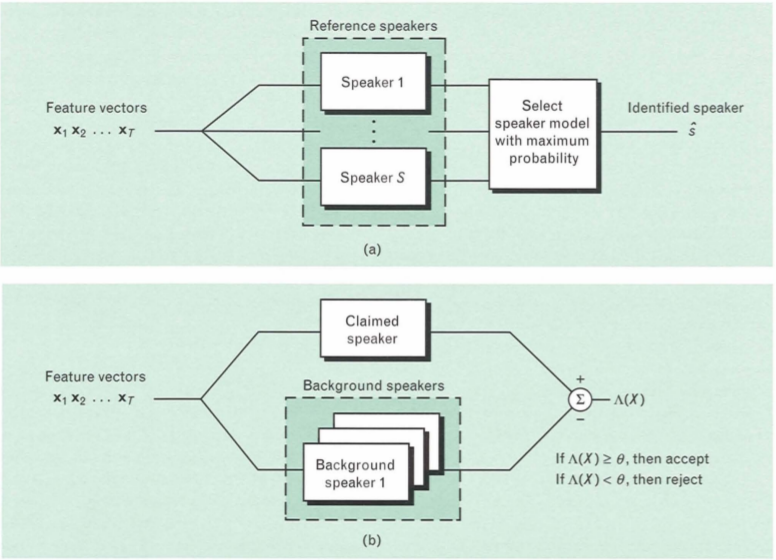
\includegraphics[width=\textwidth]{speaker-recognition-2}
    \caption{Speaker-recognition systems for (a) identification and (b) verification \cite{reynolds.1995a}.}
    \label{fig:speaker-recognition-2}
\end{figure}

Text-independent recognition is less problematic than the previous one for several reasons. First, the designer does not need to worry about what the speaker will say, since it is a vocal sound. The recognition is performed over the unique features of each vocal tract, shown when the person speaks. Second, for being free of time constraints, a HMM of single state (i.e. a GMM) fits well for the task \cite{hebert.2008}. Third, the ability to apply text-independent verification to unconstrained speech encourages the use of audio recorded from a wide variety of sources (e.g., speaker indexing of broadcast audio or forensic matching of law-enforcement microphone recordings) \cite{reynolds.campbell.2008}.

As stated in \sectionref{speaker-recognition}, the focus of this paper is in text-independent speaker verification, and due to that it is necessary to understand what is the likelihood ratio test and how the models are trained and tested.

\section{Basic Speaker Verification Architecture}

The architecture of a speaker verification system is pretty basic. Given a speech signal from a speaker $\mathcal{S}$ who claims to be a particular speaker $\mathcal{S}_i$ from a set of enrolled speakers $\boldsymbol{\mathcal{S}} = \{\mathcal{S}_1, ..., \mathcal{S}_S\}$, the strength of the claim resides on how similar the features $\boldsymbol{X}$, extracted from the speech $\boldsymbol{Y}$ produce by $\mathcal{S}$, are to the features from $\mathcal{S}_i$ ``memorized" by the system (see \equationref{decision_speaker_verification}). However a subset of enrolled speakers may have vocal similarities, leading to a misclassification of one enrolled speaker as another (a false positive). To reduce the error rate, the system must decide not only if a speech signal came from the claimed speaker, but also if it came from a background composed of all other enrolled speakers. For this, a likelihood ratio test is performed.

\subsection{Likelihood Ratio Test}

Given the speech signal $\boldsymbol{Y}$, and assuming it was produced by only one speaker, the detection task can be restated as a basic test between two hypoteses \cite{reynolds.1995b}:

\begin{description}\itemsep0pt
    \item $H_0$: $\boldsymbol{Y}$ is from the claimed speaker $\mathcal{S}_i$;
    \item $H_1$: $\boldsymbol{Y}$ is \underline{not} from the claimed speaker $\mathcal{S}_i$.
\end{description}

\noindent The optimum test to decide which hypotesis is valid is the \textbf{likelihood ratio test} between both posterior probabilities $P(H_0|\boldsymbol{Y})$ and $P(H_1|\boldsymbol{Y})$,

\begin{equation}
    \frac{P(H_0|\boldsymbol{Y})}{P(H_1|\boldsymbol{Y})} \verifytestB{\theta}{H_0}
    \label{eq:likelihood-ratio-test}
\end{equation}

\noindent where the decision threshold for accepting or rejecting $H_0$ is $\theta$. Applying Bayes' rule

\begin{equation}
    P(H_i|\boldsymbol{Y}) = \frac{p(\boldsymbol{Y}|H_i)P(H_i)}{p(\boldsymbol{Y})},
    \label{eq:bayes-for-hypotesis}
\end{equation}

\noindent and considering all hypoteses equally probable \textit{a priori}, \equationref{likelihood-ratio-test} can be simplified to

\begin{equation}
    \frac{p(\boldsymbol{Y}|H_0)}{p(\boldsymbol{Y}|H_1)} \verifytestB{\theta}{H_0}
    \label{eq:likelihood-ratio-test-2}
\end{equation}

\noindent where $p(\boldsymbol{Y}|H_i), i = 0, 1,$ is the probability density function for the hypothesis $H_i$ evaluated for the observed speech segment $\boldsymbol{Y}$. \figureref{likelihood-ratio-detector} shows the basic components found in speaker verification systems based on likelihood ratios. The front-end processing module extracts features $\boldsymbol{X} = \{\boldsymbol{x}_1, ..., \boldsymbol{x}_T\}$ (where $\boldsymbol{x}_t$ is the feature indexed at discrete time $t \in [1, 2, ..., T]$) from the speech signal $\boldsymbol{Y}$, and feeds it to the models for the hypotesized speaker and the background. The hypoteses $H_0$ and $H_1$ are represented mathematically by models detoned $\lambda_{hyp}$ and $\lambda_{\overline{hyp}}$, respectively. The likelihood equation from \equationref{likelihood-ratio-test-2} is be better represented as

\begin{equation}
    \frac{p(\boldsymbol{X}|\lambda_{hyp})}{p(\boldsymbol{X}|\lambda_{\overline{hyp}})} \verifytest{\theta}{\mathcal{S} \text{ as } \mathcal{S}_i}
    \label{eq:likelihood-ratio-test-3}
\end{equation}

The division seen in \equationref{likelihood-ratio-test-3} can be transformed in a subtraction by the application of the logarithm function. Since the logarithm is monotonically increasing, the behavior of the likelihood ratio is maintained, and \equationref{likelihood-ratio-test-3} is replaced by the log-likelihood ratio

\begin{equation}
    \Lambda(\boldsymbol{X}) = \log p(\boldsymbol{X}|\lambda_{hyp}) - \log p(\boldsymbol{X}|\lambda_{\overline{hyp}})
    \label{eq:log-likelihood-ratio}
\end{equation}

\noindent The more likely $\mathcal{S}$ is of $\lambda_{hyp}$ and the less likely $\mathcal{S}$ is of $\lambda_{\overline{hyp}}$ easier is to accept $\mathcal{S}$ as the claimed $\mathcal{S}_i$.

\begin{figure}[ht]
    \centering
    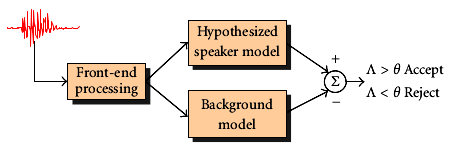
\includegraphics[width=0.75\textwidth]{likelihood-ratio-detector}
    \caption{Likelihood ratio-based speaker detection system \cite{bimbot.et.al.2004}.}
    \label{fig:likelihood-ratio-detector}
\end{figure}

\subsection{Training Phase}

Once the features are extracted from the speech signal, they are used to train the models $\lambda_{hyp}$ and $\lambda_{\overline{hyp}}$. A high-level demonstration of the training of $\lambda_{hyp}$ (mathematical representation of $\mathcal{S}_i$) is shown in \figureref{speaker-verification-training}.

\begin{figure}[ht]
    \centering
    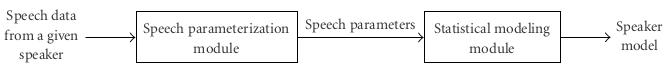
\includegraphics[width=\textwidth]{speaker-verification-training}
    \caption{The statistical model of $\mathcal{S}$ is created from the features $\boldsymbol{X}$ \cite{bimbot.et.al.2004}.}
    \label{fig:speaker-verification-training}
\end{figure}

\noindent Due to $\lambda_{hyp}$ be a model of $\mathcal{S}_i$, the features used to train it (i.e., estimate $p(\boldsymbol{X}|\lambda_{hyp})$) are extracted from speech signals produced by $\mathcal{S}_i$. For $\lambda_{\overline{hyp}}$ the same process is executed, considering it a representation of another speaker (i.e., the \emph{mirror} of $\mathcal{S}_i$).

The model $\lambda_{\overline{hyp}}$ is not well-defined. It is composed of the features extracted from speech signals from all other speakers except $\mathcal{S}_i$. One popular approach to deal with this difficulty is to define the likelihood of $\lambda_{\overline{hyp}}$ as

\begin{equation}
    p(\boldsymbol{X}|\lambda_{\overline{hyp}}) = \mathcal{F}[p(\boldsymbol{X}|\lambda_1), ..., p(\boldsymbol{X}|\lambda_S)],
    \label{eq:log-likelihood-ratio}
\end{equation}

\noindent where $\mathcal{F}$ is a function of all likelihoods of set $\boldsymbol{\mathcal{S}}$ (except $\mathcal{S}_i$), such as mean or maximum. In various contexts, this set of other speakers has been called likelihood ratio sets, cohorts, and background speakers \cite{reynolds.quatieri.dunn.2000}.

Another popular approach is to create only one model for $\lambda_{\overline{hyp}}$, containing features extracted from speeches of all enrolled speakers (even the claimed $\mathcal{S}_i$). The weight of $\mathcal{S}_i$ in $\lambda_{\overline{hyp}}$ is reduced due to the presence of all other speakers from $\boldsymbol{\mathcal{S}}$. This model is named \textbf{Universal Background Model} (UBM) and is denoted by $\lambda_{bkg}$. \equationref{likelihood-ratio-test-3} is rewritten as

\begin{equation}
    \frac{p(\boldsymbol{X}|\lambda_{hyp})}{p(\boldsymbol{X}|\lambda_{bkg})} \verifytest{\theta}{\mathcal{S} \text{ as } \mathcal{S}_i}
    \label{eq:likelihood-ratio-test-4}
\end{equation}

\noindent The UBM is explained in details in \chapterref{gmm}.

\subsection{Test Phase}

As seen in \equationref{likelihood-ratio-test-4}, the decision process is based on a function \emph{Score} calculated from the likelihood ratio of $p(\boldsymbol{X}|\lambda_{hyp})$ and $p(\boldsymbol{X}|\lambda_{bkg})$. Being the vector of features $\boldsymbol{X} = \{\boldsymbol{x}_1, ..., \boldsymbol{x}_T\}$, with all $\boldsymbol{x}_t$ independent of the others, the likelihood of a model $\lambda$ given $\boldsymbol{X}$ can be written as

\begin{equation}
    p(\boldsymbol{X}|\lambda) = \prod_{t=1}^T p(\boldsymbol{x}_t|\lambda).
    \label{eq:likelihood-prod}
\end{equation}

\noindent Using the logarithm function, \equationref{likelihood-prod} becomes

\begin{equation}
    \log p(\boldsymbol{X}|\lambda) = \frac{1}{T} \sum_{t=1}^T \log p(\boldsymbol{x}_t|\lambda),
    \label{eq:log-likelihood-sum}
\end{equation}

\noindent where the term $\frac{1}{T}$ is used to normalize the log-likelihood to the duration of the speech signal. That said, the likelihood ratio given by \equationref{likelihood-ratio-test-4} becomes a subtraction

\begin{equation}
    \text{\emph{Score}}(\boldsymbol{X}) = \log p(\boldsymbol{X}|\lambda_{hyp}) - \log p(\boldsymbol{X}|\lambda_{bkg}),
    \label{eq:score_of_X}
\end{equation}

\noindent with \emph{Score}$(\boldsymbol{X})$ being compared to $\log\theta$ and maintaining the same rule from \equationref{likelihood-ratio-test-4}.